\captionsetup[subfigure]{justification=centering}
    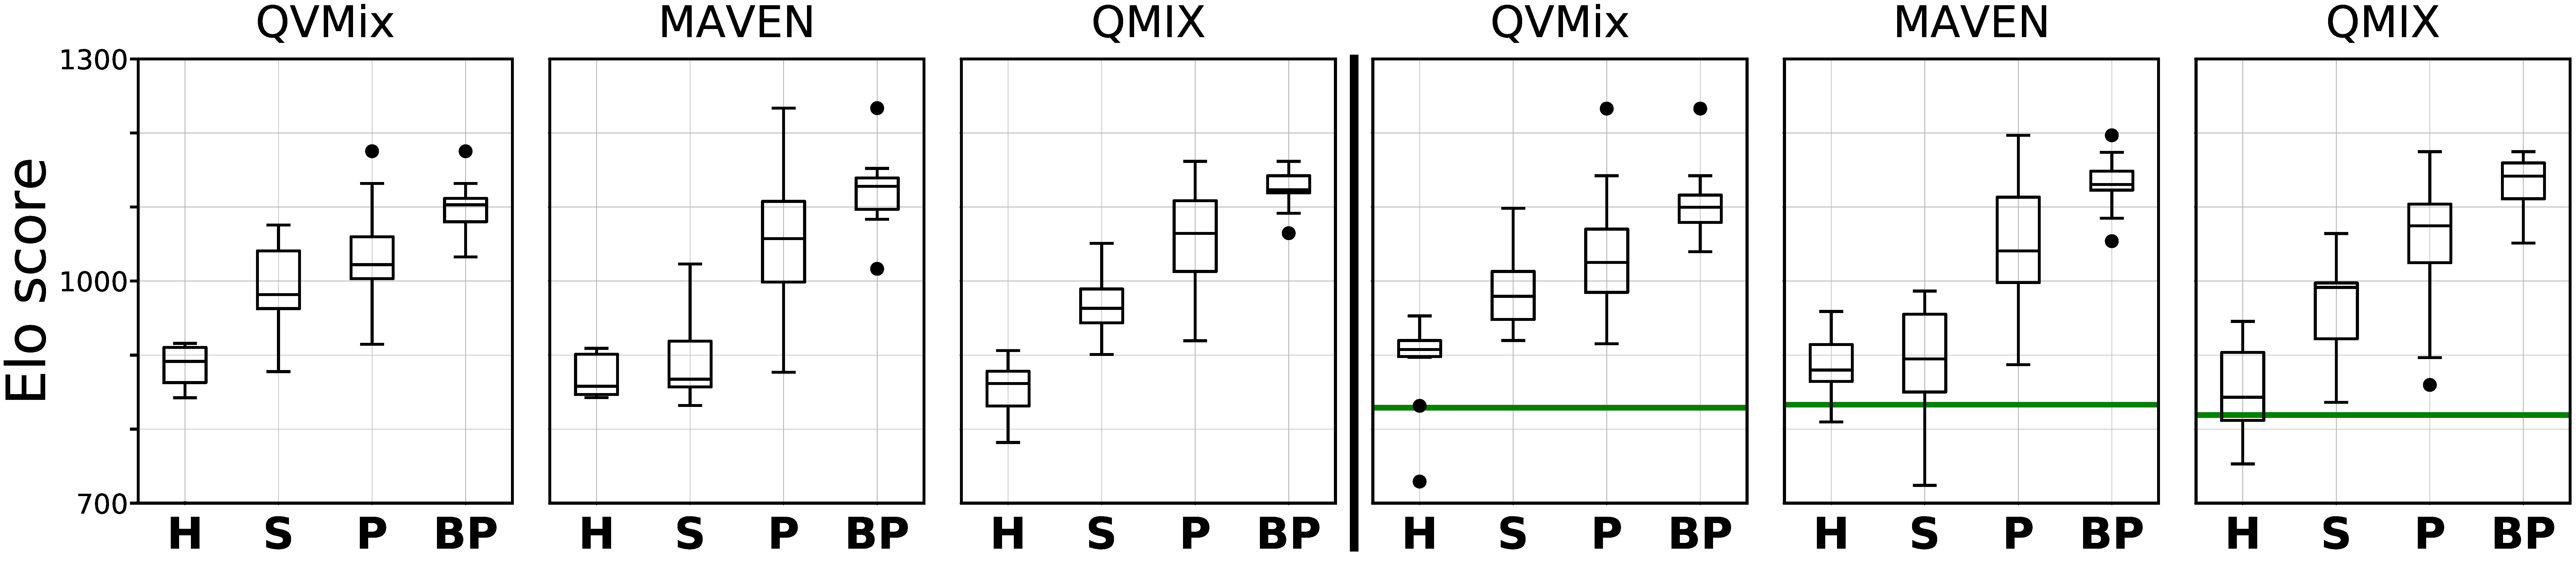
\includegraphics[width=\textwidth]{tex_thesis/figures/ch7/3m_tiny_six_qvmix_maven_qmix.pdf}
    \begin{subfigure}{.045\textwidth}
    \centering
    \caption*{}
    \end{subfigure}%
    \begin{subfigure}{.455\textwidth}
        \begin{subfigure}{.33\textwidth}
            \renewcommand\thesubfigure{\alph{subfigure}.1}
          \centering
          \caption{}
          \label{subfig:elo_no_h_methodQVMIX}
        \end{subfigure}%
        \begin{subfigure}{.33\textwidth}
        \addtocounter{subfigure}{-1}
            \renewcommand\thesubfigure{\alph{subfigure}.2}
          \centering
          \caption{}
          \label{subfig:elo_no_h_methodMAVEN}
        \end{subfigure}%
        \begin{subfigure}{.33\textwidth}
        \addtocounter{subfigure}{-1}
            \renewcommand\thesubfigure{\alph{subfigure}.3}
          \centering
          \caption{}
          \label{subfig:elo_no_h_methodQMIX}
        \end{subfigure}%
    \centering
    \addtocounter{subfigure}{-1}
    \caption{$3m$ map \textbf{without} heuristic.}
    \label{subfig:elo_no_h_3m}
    \end{subfigure}%
    \begin{subfigure}{.455\textwidth}
        \begin{subfigure}{.33\textwidth}
        \renewcommand\thesubfigure{\alph{subfigure}.1}
          \centering
          \caption{ }
          \label{subfig:elo_h_methodQVMIX}
        \end{subfigure}%
        \begin{subfigure}{.33\textwidth}
         \addtocounter{subfigure}{-1}
        \renewcommand\thesubfigure{\alph{subfigure}.2}
          \centering
          \caption{ }
          \label{subfig:elo_h_methodMAVEN}
        \end{subfigure}%
        \begin{subfigure}{.33\textwidth}
            \addtocounter{subfigure}{-1}
            \renewcommand\thesubfigure{\alph{subfigure}.3}
          \centering
          \caption{ }
          \label{subfig:elo_h_methodQMIX}
        \end{subfigure}%
    \centering
    \addtocounter{subfigure}{-1}
    \caption{$3m$ map \textbf{with} heuristic.}
     \label{subfig:elo_h_3m}
    \end{subfigure}%
    
    

    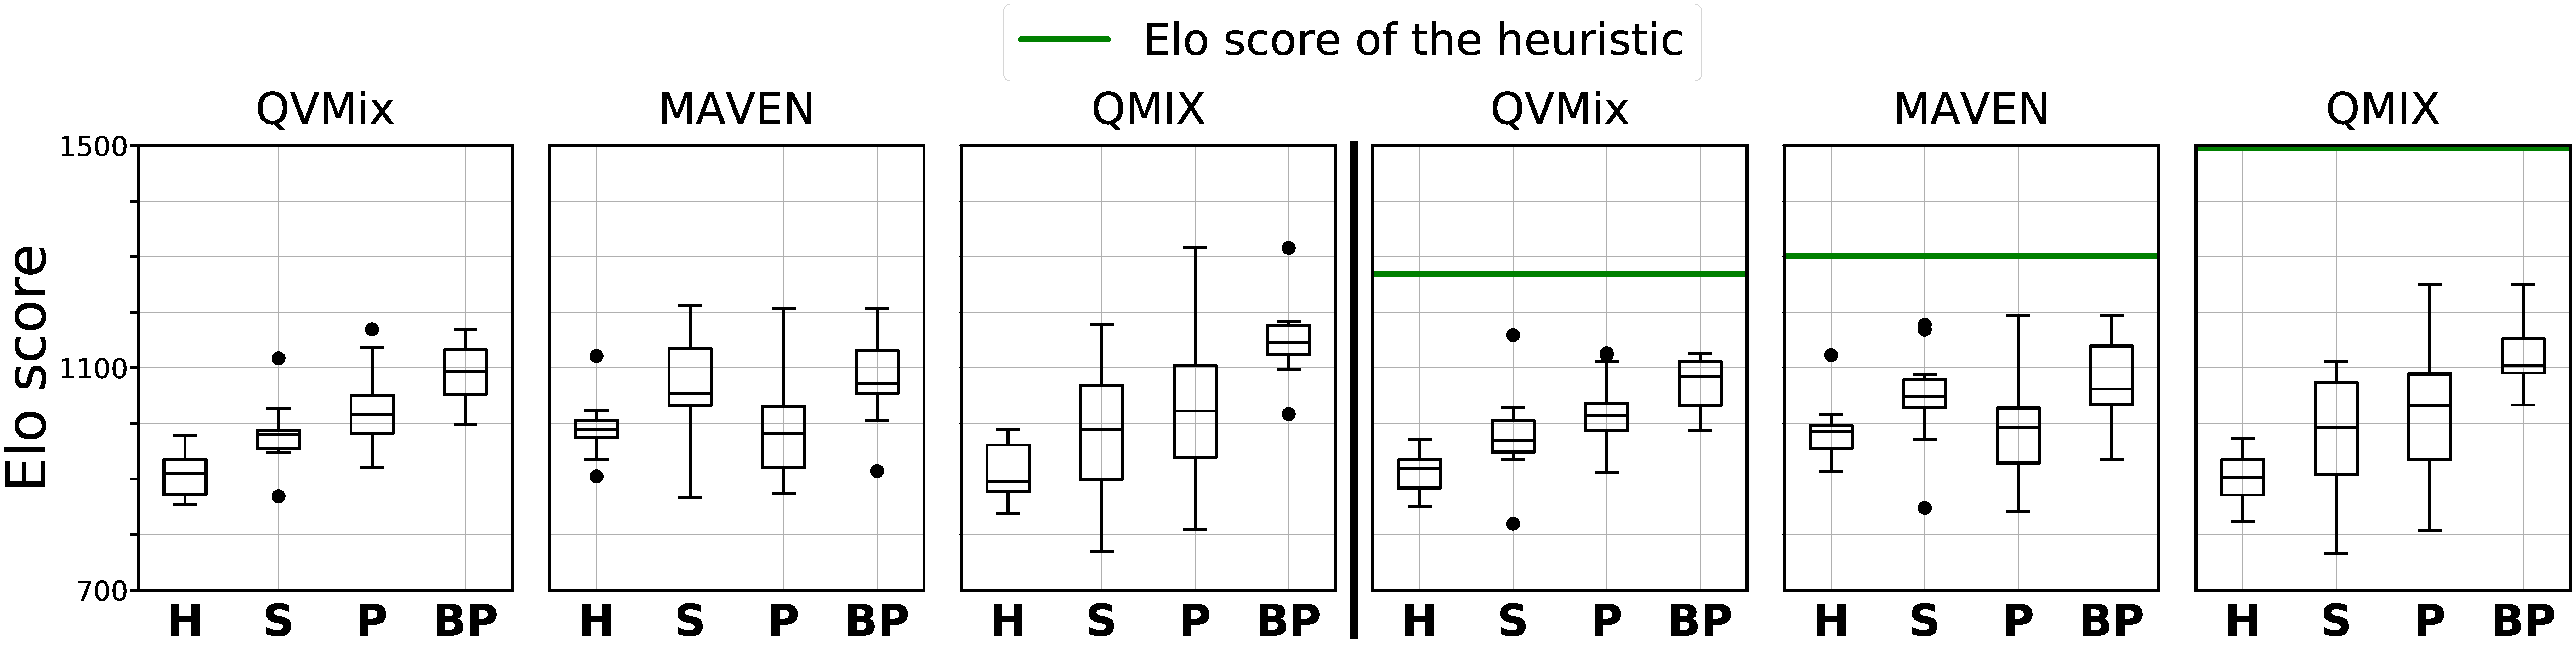
\includegraphics[width=\textwidth]{tex_thesis/figures/ch7/3s5z_tiny_six_qvmix_maven_qmix.pdf}
    \begin{subfigure}{.045\textwidth}
    \centering
    \caption*{}
    \end{subfigure}%
    \begin{subfigure}{.455\textwidth}
        \begin{subfigure}{.33\textwidth}
            \renewcommand\thesubfigure{\alph{subfigure}.1}
          \centering
          \caption{}
          \label{subfig:3s5z_elo_no_h_methodQVMIX}
        \end{subfigure}%
        \begin{subfigure}{.33\textwidth}
        \addtocounter{subfigure}{-1}
            \renewcommand\thesubfigure{\alph{subfigure}.2}
          \centering
          \caption{}
          \label{subfig:3s5z_elo_no_h_methodMAVEN}
        \end{subfigure}%
        \begin{subfigure}{.33\textwidth}
        \addtocounter{subfigure}{-1}
            \renewcommand\thesubfigure{\alph{subfigure}.3}
          \centering
          \caption{}
          \label{subfig:3s5z_elo_no_h_methodQMIX}
        \end{subfigure}%
    \centering
    \addtocounter{subfigure}{-1}
    \caption{$3s5z$ map \textbf{without} heuristic.}
     \label{subfig:elo_no_h_3s5z}
    \end{subfigure}%
    \begin{subfigure}{.455\textwidth}
        \begin{subfigure}{.33\textwidth}
        \renewcommand\thesubfigure{\alph{subfigure}.1}
          \centering
          \caption{ }
          \label{subfig:3s5z_elo_h_methodQVMIX}
        \end{subfigure}%
        \begin{subfigure}{.33\textwidth}
         \addtocounter{subfigure}{-1}
        \renewcommand\thesubfigure{\alph{subfigure}.2}
          \centering
          \caption{ }
          \label{subfig:3s5z_elo_h_methodMAVEN}
        \end{subfigure}%
        \begin{subfigure}{.33\textwidth}
            \addtocounter{subfigure}{-1}
            \renewcommand\thesubfigure{\alph{subfigure}.3}
          \centering
          \caption{ }
          \label{subfig:3s5z_elo_h_methodQMIX}
        \end{subfigure}%
    \centering
    \addtocounter{subfigure}{-1}
    \caption{$3s5z$ map \textbf{with} heuristic.}
     \label{subfig:elo_h_3s5z}
    \end{subfigure}%
    
    \caption{Elo score box plots of 12 test populations. 
    Half of the experiments were performed in the $3m$ map, shown at the top (\ref{subfig:elo_no_h_3m}, \ref{subfig:elo_h_3m}) and the other half in the $3s5z$ map, shown at the bottom (\ref{subfig:elo_no_h_3s5z}, \ref{subfig:elo_no_h_3s5z}). 
    In each test population, teams are trained with the same method, which is either QVMix (\ref{subfig:elo_no_h_methodQVMIX}, \ref{subfig:elo_h_methodQVMIX},\ref{subfig:3s5z_elo_no_h_methodQVMIX}, \ref{subfig:3s5z_elo_h_methodQVMIX}), MAVEN (\ref{subfig:elo_no_h_methodMAVEN}, \ref{subfig:elo_h_methodMAVEN},\ref{subfig:3s5z_elo_no_h_methodMAVEN}, \ref{subfig:3s5z_elo_h_methodMAVEN}) or QMIX (\ref{subfig:elo_no_h_methodQMIX}, \ref{subfig:elo_h_methodQMIX},\ref{subfig:3s5z_elo_no_h_methodQMIX}, \ref{subfig:3s5z_elo_h_methodQMIX}).
    In \ref{subfig:elo_h_3m} and \ref{subfig:elo_h_3s5z}, the heuristic is present in the test population and a green line represents its Elo score.
    Box plots represent the distribution of the ELO scores of the teams trained either against the heuristic (\textbf{H}), in self-play (\textbf{S}), within a population (\textbf{P}) or the best of each training population (\textbf{BP}).
    For most methods, teams trained within a population achieved the highest Elo scores.
    Box plots present the median, the first quantile ($Q1$) and the third quantile ($Q3$). The reach of whiskers is defined by $1.7*(Q3-Q1)$.
    }
    \label{fig:elo_method}

